
\begin{frame}

    \frametitle{Why does QUIC exist?}

    \note{Well, QUIC started with HTTP/2.}

    \begin{overprint}
        \uncover<+->{}
        \uncover<+->{
        HTTP/2 was created in order to shorten web latencies. HTTP/2 removes the limitation of HTTP/1.1 which only can send one resource at the time over a TCP connection. }
        ~\\
        ~\\
        \uncover<+->{
        Sending multiple resources over the same TCP connection is both what makes HTTP/2 perform better AND worse than HTTP/1.1.}
    \end{overprint}

\end{frame}

% -------------------------------------------

\begin{frame}
    \frametitle{Why does QUIC exist?}
    \begin{overprint}
        \framesubtitle{What? This makes no sense?}

        \uncover<+->{}
        \uncover<+->{
        On stable connections HTTP/2 performs objectively better when fetching many resources. In \href{https://http2.akamai.com/demo}{some edge cases} a lot better.}
        ~\\
        ~\\
        \uncover<+->{
        In most web browsing however the user can't notice the difference because of processing delay from their browser.}

        \note{According to Bocchi et al. This is a combination of actual processing delay limitations and that many web pages are optimized to work well with HTTP/1.1}


    \end{overprint}

\end{frame}

% -------------------------------------------
\begin{frame}
    \frametitle{Why does QUIC exist?}
    \framesubtitle{What about not so stable connections then?}

        \only<2>{
        Sending multiple resources over one TCP connection becomes a problem. A packet-loss or out-of-order packet for one resource stream causes head-of-line blocking.}

\end{frame}

% ----------------------------------

\begin{frame}
    \frametitle{Why does QUIC exist?}
    \framesubtitle{What about not so stable connections then?}
    \begin{overprint}

        \uncover<+->{}
        \only<2>{
        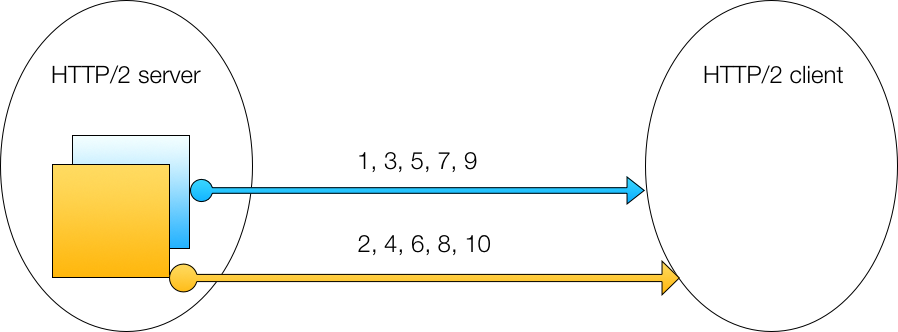
\includegraphics[width=0.9\textwidth]{figures/http2-two-resources.png}}
        \only<3,4>{
        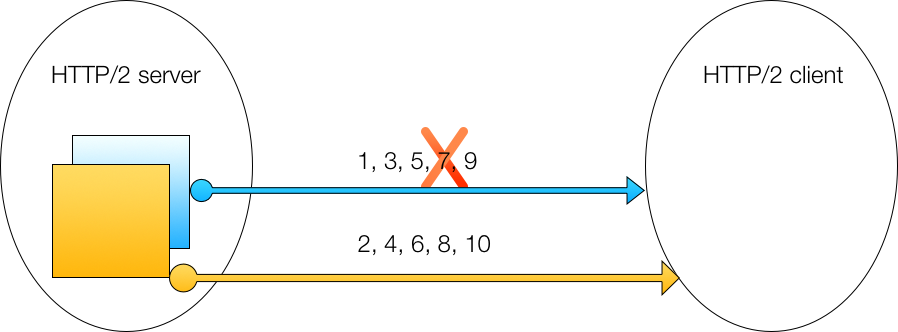
\includegraphics[width=0.9\textwidth]{figures/http2-two-resources-packet-loss.png}}
        \only<4>{
        Head-of-line blocking is introduced since the TCP connection counts every packet with a index higher than the lost packet as ``not arrived yet''.}

    \end{overprint}

\end{frame}


% ----------------------------------
\begin{frame}
    \frametitle{Why does QUIC exist?}
    \framesubtitle{QUIC improvements over HTTP/2}

    \begin{overprint}
        \uncover<+->{}

        \begin{itemize}
            \uncover<+->{
            \item QUIC includes per-stream congestion control, avoiding head-of-line blocking.}
            \uncover<+->{
            \item QUIC has way faster connection setup times (0-1 RTT vs 3 RTT).}
            \uncover<+->{
            \item Connection migration. Allows connection to continue even if user changes IP-address (moving between LTE/WiFi for example).}
            \uncover<+->{
            \item Forward error correction.}
        \end{itemize}

    \end{overprint}

\end{frame}

